\documentclass[conference]{IEEEtran}
\IEEEoverridecommandlockouts
% The preceding line is only needed to identify funding in the first footnote. If that is unneeded, please comment it out.
\usepackage[superscript]{cite}
\usepackage{url}
\usepackage{amsmath,amssymb,amsfonts}
\usepackage{algorithmic}
\usepackage{graphicx}
\usepackage{textcomp}
\usepackage{xcolor}
\usepackage{hyperref}
\usepackage{xcolor}
\hypersetup{
    colorlinks,
    linkcolor={red!50!black},
    citecolor={blue!50!black},
    urlcolor={blue!80!black},
}

\def\BibTeX{{\rm B\kern-.05em{\sc i\kern-.025em b}\kern-.08em
    T\kern-.1667em\lower.7ex\hbox{E}\kern-.125emX}}
\begin{document}

\title{Phishing Detection in Browsers \linebreak using Machine Learning\\
}

\author{\IEEEauthorblockN{Tanmay Naik}
    \IEEEauthorblockA{\textit{Khoury College of Computer Sciences} \\
        \textit{Northeastern University}\\
        Boston, US \\
        naik.t@northeastern.edu}
    \and
    \IEEEauthorblockN{Nithin Gangadharan}
    \IEEEauthorblockA{\textit{Khoury College of Computer Sciences} \\
        \textit{Northeastern University}\\
        Boston, US \\
        gangadharan.n@northeastern.edu}

}

\maketitle

\begin{abstract}
    % From the report requirement:
    % The abstract should consist of at most 2 paragraphs and must discuss: a) the project’s motivation, i.e.why the problem and the proposed solution are important, b) the proposed approach from a high-level point of view, and c) the most important results and findings.

    Phishing is a cybercrime in which a target visits a website that is posing as a legitimate application, to lure individuals into providing sensitive data such as - banking and credit card details, and passwords.
    An unsuspecting user can click a link in an email or social media platform, and be led to a phishing website, which may lead to fraud and identity theft.
    Phishing is a widespread attack that still does not have a concrete solution.
    \par This report proposes a solution for the protection of end users through a browser extension while comparing various Machine Learning approaches to identify phishing websites.
    Rule-based approaches can be limiting since there are new phishing websites created everyday. Machine Learning based approaches aim to solve that, with the trade-off being that results will be probabilistic rather than absolute. Experiments described in this report use a combination of these methods, which results in a model that serves the purpose well and requires little overall maintenance in the long run.
\end{abstract}

% \begin{IEEEkeywords}
%     component, formatting, style, styling, insert
% \end{IEEEkeywords}

\section{Introduction}
% From the report requirement:
% Introduction [≈0.5 page] is commonly an extended version of the abstract. Therefore, these topics should be discussed  in  the  introduction:  a)  the  problem  that  is  intended  to  be  solved  in  this  project  and motivating the problem by elaborating on its importance, b) the proposed approach in an explicit way, i.e. what are the exact inputs and outputs to the proposed solution and how they are processed, c) a summary of experimental results which is more fine-grained than abstract.

With the recent advancement in various cybersecurity technologies, the weakest link in  cybersecurity happen to be the end users.
Attackers utilize phishing which exploits naivety of users to trick them into handing out sensitive information.
This poses a great risk not only to the users themselves but the organizations and institutions of which they are a part of.
According to recent research from Proofpoint, 75\% of organizations around the world experienced a phishing attack in 2020, and 74\% of attacks targeting US businesses were successful \cite{stateofphishing}.

\par Most of the software interactions between users and organizations happen through websites on computers/laptops. Forcing users to install a custom application to be run is a rarity due to the convenience a browser provides. Web-based security for browsers are crucial in current day and Phishing is one of the crimes that still exists.

\par Apart from increasing security awareness among users, the tools which complement that awareness to help users make safe decisions must be developed.
This report proposes and demonstrates a Chromium-based browser extension to help mitigate the risk of phishing while browsing the web.
The central idea of the browser extension is to notify the user whenever they open any \emph{potential} phishing website.

\par The solution also includes a Python web server which utilizes various Machine Learning classification techniques to determine the legitimacy of the webpage in question.
The web server takes in a URL and returns a boolean value indicating if the given URL is part of a potential phishing attempt.

\par The browser extension monitors each URL that the user visits, and tries to determine if the URL is malicious with the help of the web server.
The web server exposes a REST API which is consumed by the extension for communication.
The same API can also be reused as-is to implement a similar phishing detection in a different context like a network-level application or in a mobile application like Android.

\par The server implements both a mixture of rule based approach and Machine Learning classification techniques. The rule based approach is useful to weed out obvious URLs and is rather an inexpensive operation. The Machine Learning classification techniques is more expensive to do, but helps predict whether a URL can be a phishing site.

\section{Related Work}
% From the report requirement:
% [≈ 0.5 page]In this section, similar approaches that have been proposed for the same problem in the project
% should be discussed. In particular, the advantages and disadvantages of these approaches should be
% summarized in this section. It is required to have at least 5 related works and references in this
% section that have been published in top venues. Google Scholar is the best search engine to find
% similar works
\paragraph{PhishDetector\cite{PhishDetector}}
This is a Chromium extension which has set out to solve exactly the same problem as this project.
Based to its description on the website and the analysis of its behavior, it can be concluded that this extension uses a rule-based system to determine if a webpage is a phishing attempt.
It also seems to be particularly accurate when it comes to identifying illegitimate banking pages.
Even though rule-based systems are great for detecting simple phishing attempts, they are not ideal for more sophisticated phishing attempts.
Rule-based systems are also inherently complex to maintain - adding and modifying rules over time makes the system more complex and unmanageable with time.
They also demand more human intervention to define the rules and for their maintenance.
Using Machine Learning in lieu of rule-based system gets rid of many of these limitations.
As Machine Learning is data centric, it doesn't require managing complex rules and makes it straightforward to tweak the algorithms.

\paragraph{Cloudphish\cite{Cloudphish}}
Cloudphish is a phishing detector for web-based email software.
It monitors all emails received by a user and checks each email for a phishing attack.
Having a paid subscription model, it offers a \emph{decent} service.
But the major limitation it has is that it works only with the email inbox.
Even though many of the phishing attacks are carried over through email, phishing is as prominent on social media and messaging apps in this age.
And that calls for a solution which monitors all the web activity to identify phishing attacks regardless of their method of delivery.

\par There are various other browser extensions which virtually have the same limitations as the aforementioned solutions\cite{BlueArca}\cite{Retruster}\cite{PhishingBoat}
As their limitations are encompassed in the discussion of other solutions above, their detailed discussion has been omitted for brevity.

\par To summarize, there are various browser plugins consisting of rule-based systems, simple whitelists-blacklists and some even making use of Machine Learning and Artificial Intelligence. But there needs to be a solution which utilizes all available phishing detection methods to protect the average internet user from criminals.

\section{Approach}
% From the report requirement:
% [≈ 1 to 1.5 pages]
% This section should present your approach in detail. Note that although the teaching staff may 
% know this approach, other readers may not. Thus, please, provide a description of how the applied 
% method works. Also, it is strongly recommended to include a figure that shows the overall 
% architecture of your solution.
The architecture of this project consists of two primary components: The browser extension and the web server.

\paragraph{Browser Extension}
The extension is developed for Chromium-based browsers using JavaScript with HTML and CSS.
Therefore it is compatible with any Chromium implementation including Google Chrome, Microsoft Edge, Brave, etc.
The extension monitors each web page that is visited by the user and fetches the URL of that webpage.
It then communicates with the web server which tells if the given URL is part of a phishing attempt or not.
The user is notified with the results of the analysis based on the response from server.
The extension will stay silent in the background while the user is visiting websites that it has deemed safe.
It only \emph{bothers} them when there is a potential of phishing on the site they are currently visiting help them make a safer decision.

\paragraph{Python Web Server}
The web server has an REST endpoint which takes in a URL and uses Machine Learning techniques to classify it into categories.
It extracts relevant ``features'' from the URL and feeds them to \emph{Classification Models} to determine the legitimacy of the URL.
This process is expanded upon further down in this section.

\begin{figure}[htbp]
    \centerline{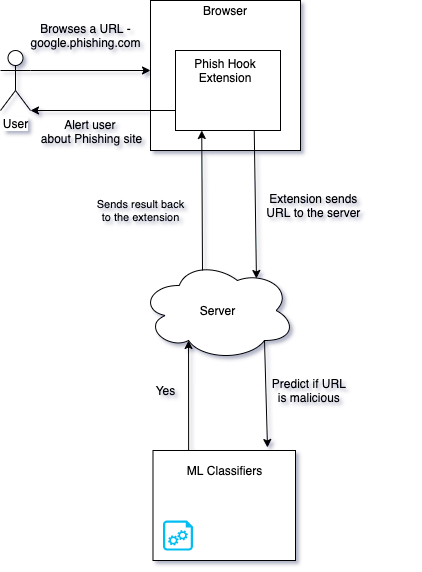
\includegraphics[scale=.5]{phish-arch.png}}
    \caption{Architecture overview of the application}
    \label{fig}
\end{figure}

\par Classification is a process of categorizing a given set of data into classes.
In this case, there would be two classification labels: ``spam'' and ``not spam''.
And the input data would be values of various features of the URL which are deemed effective for high quality classification of any URL into one of the classes.


\par The process of creating a classification model consists of two primary stages.
The first is the training stage where a classifier is fed a large amount of input with along with their respective class labels.
That creates a classification model which is given a set of inputs without their respective labels to let it classify each input to a class.
That constitutes the second stage where the correctness of the newly created classification model is compared against the actual labels.
The input set given to the model for the second stage is often referred to as \emph{testing dataset} and the data used for the first stage is called \emph{training dataset}.
As a common practice, the dataset on hand is split into training and testing datasets for creation and testing of the classification models, respectively.

\par The classifiers used in this project are described below:
\begin{enumerate}
    \item Decision Trees:
          Decision Trees belong to the family of supervised machine learning algorithms.
          Decision trees classify the input by running them down the tree from the root node to some leaf node, whereas the leaf node provides the classification of the input.
    \item K-Nearest Neighbors (KNN):
          The KNN algorithm assumes that similar things are \emph{near} to each other.
          Based on this assumption, it classifies all nearby data points into one.
          Then, it classifies the given input by locating N-nearest neighbors and finding mode of their labels which is predicted to be the label of the input set.
    \item Random Forests:
          Random Forests consist of a large number of Decision Trees that operate as an ensemble.
          Each tree in a forest classifies the given input set to a label and the label with the highest number of votes is considered as the prediction of the Random Forest.
          \par The individual trees in a random forest are relatively \emph{uncorrelated}, and they perform better as an ensemble than they would on their own.
          To put it in layman's terms, the trees safeguard each other from their individual errors.
\end{enumerate}

\par The following section describes the datasets used for training and testing the models with the aforementioned classifiers.
\begin{enumerate}
    \item Phishing Websites Dataset\cite{UCIDataset}:
          This dataset has 11,055 datapoints with 6,157 legitimate URLs and 4,898 phishing URLs.
          And it contains 30 features subdivided into three categories:
          \begin{enumerate}
              \item Features based on the domain and subdomains
              \item Features derived from the other parts of the URL
              \item Features derived from the webpage HTML and JavaScript
          \end{enumerate}
    \item Datasets for phishing websites detection\cite{GregaDataset}:
          This dataset consists of 111 features, of which 97 are based on the URL.
          For the phishing websites, the list was extracted from the PhishTank registry which are verified by multiple users.
          And for sets of legitimate websites, the publicly available and community labeled lists are utilized\cite{citizenlablists}.
\end{enumerate}

\par When the server receives the URL, before it can be tested by any of the Machine Learning models, it are checked against a whitelist.
The whitelist is extracted from The Majestic Million dataset\cite{MajesticMillion} which maintains a list of top 1 million domains on the internet.
The whitelist helps in reducing the processing and network overhead of checking the most popular sites which would be visited by an average user on a day to day basis. The experiments sections further elaborates on the need for doing this.

\par The machine learning models are already trained with both datasets, are precomputed and stored on the server.
If the given domain is not part of the whitelist, the URL is then passed on to these models.
Whenever the server receives a URL to be tested, it extracts all the features from the given URL.
Many of the features are extracted through string parsing and the rest of them require use of external APIs and libraries.
For example, PageRank of a given domain is fetched using Open PageRank API\cite{OpenPageRank}.

\par After extracting the relevant features for each dataset, they are passed on to the classification models and their ensembles.
And the result is sent back based on the outputs of the various models. 
One advantage of using a server based approach is essentially, results for different URLs from different users can be cached. This can save recurring computation for the same URL across users and decreases response times on repeated requests.


\section{Experiments and Results}
% [≈ 1 to 3 pages]
% All experimental settings and results are discussed in this section. For example, you should explain
% about the system’s configuration where you conducted the experiments or, discuss about which the 
% programming language that you used to implement the proposed solution. Also, you should provide 
% a link to a repository (e.g., a Github repo) where your implementation could be downloaded and 
% evaluated. 

Experiments in this report mainly concern 2 things - Effectiveness and Efficiency of Phishing detection. Due to the nature of the problem, the focus was more on effectiveness since there were a lot of parameters to tune. That being said, efficiency concerns are legitimate and were explored as well.

\par One of the important characteristics of a machine learning model is the data-set that is used to train it. The nature of the data-set greatly impacts the effectiveness of the result. Initially, Experiments were done on various data-sets that were available across the web using simple classification methods and the accuracy results were compared to the filter out the ineffective collections.

\par The decision to use two data-sets as a part of the final application was based on the observation that "Phishing Websites Dataset"\cite{UCIDataset} had a lot of non-url based features that which worked very well based off of the content of the website. In contrast, "Datasets for Phishing websites detection"\cite{GregaDataset} data-set contains 97 features that depended only on the URL structure, which are effective in detecting phishing websites. The inclusion of both these data-sets, with the result from their combined models, effectively acts as a way for the result to have legitimate checks and balances as well. If both the models predict that a website might be a phishing website, there is a high probability that it is true. Whenever there is a partial agreement, it is prudent to let the user know and be the final-arbiter of this conflict. This exploration allowed the feature of "Caution" vs "Alert" notifications to come up organically.

\par The models were built by splitting a portion of the input as training and test data, using a Decision Tree classifier and cross-validated into 10 splits. It was verified manually by using it as an extension in regular day-to-day browsing, to flag obvious errors. For the model from the dataset "Datasets  for  phishing  websites  detection"\cite{GregaDataset}, it was noticed that the accuracy of the model was high with the test data, but performed rather poorly with random samples from the real world. This lead to the hypothesis that the model was over-fitting the data-set. This lead to the introduction of the ensembles for this model in particular. The combination of additional classifiers were tried out (Decision Tree, k-Nearest Neighbors and Random Forest) and verified with the same methods, until a minimum accuracy of 80\% was achieved.

\par Tuning individual classifiers is also detrimental to the overall accuracy measurement of a model. For the "Datasets  for  phishing  websites  detection"\cite{GregaDataset} model, the classification-ensemble contained a K-Nearest Neighbor classifier. The number of neighbors for the classification was increased to the effect, that it over-fit the data. This was fruitful, since the ensemble of different classifiers helped reduce overall variance of the model.

\par The above experiments were predominantly effectiveness-based approaches. Although using a combination of two models helped improve the overall goal of detecting phishing websites, it came at the cost of the delay in prediction. Steps were taken to parallelize the flow of aggregating the predictions from the two models. That being said, there is no denying the fact that using a classifier to predict outcomes is inherently an expensive process. In a resource constrained environment, it must be called upon only when truly necessary. And once it's called upon, it is prudent for its results to be reused, to save the cost of classifying again. To this effect, a "Whitelist" of frequently used websites was added to skip prediction entirely, for overtly obvious websites. Since the intended application of this classification is in browser extensions,  the fact that users will browse popular websites frequently is not an entirely unfair assumption. Caching the results on the server also goes well with this approach. This rule-based counterpart for the Machine Learning classifier helps improve the overall efficiency of the server.

\begin{table}[htbp]
    \caption{Performance Results of the Models}
    \begin{center}
    \begin{tabular}{|c|c|c|c|c|}
    \hline
    \textbf{Model} & \textbf{Accuracy}& \textbf{Precision}& \textbf{Recall}& \textbf{F1 Score} \\
    \hline
    Ensemble Model\cite{GregaDataset}& 90.68& 92.69 & 89.20 & 90.92\\
    \hline
    Decision tree Model\cite{UCIDataset}& 80.37& 84.03 & 80.82 & 82.40 \\
    \hline
    \end{tabular}
    \label{tab1}
    \end{center}
    \end{table}
    

\par The implementation of the report can be found in this repository, which contains the source-code as well as steps to get it running on a local machine - \href{https://github.com/gnithin/phish-hook}{https://github.com/gnithin/phish-hook}

\section{Conclusion and Future Work}
% [≈ 1 to 2 paragraphs]
% You should summarize your entire report in this section by reiterating key points. Also, you should 
% explicitly and briefly explain how the current work could be improved in future research projects
\par Phishing is one of the most widespread security attacks on the internet of this age.
As the attacks keep getting more and more sophisticated, the solutions to prevent them need to keep with them.
The traditional methods to detect attacks need to be combined with the growing fields of machine learning and artificial intelligence.
It is apparent from various experiments and observations that the ideal solution to such issues, if any, is to combine best of all approaches and make them work with each other.

\par For the enhancement of this implementation, there seems to be a potential to improve the machine learning models as well as the features that are being used for classification.
The extension and the server can be updated to also take in user feedback regarding a misclassification of any site.
And the feedback would be considered by the classification models to improve their performance.
Although, it might introduce a fresh set of challenges such as abuse of the feedback system to pass off an illegitimate site as safe (adversarial attacks).
Potential solution to this problem would be to have a threshold on number of feedbacks until which the system does not consider them for the particular website.

\par The solution proposed and implemented in this project can be a genesis to a series of tools and products which strive to solve the issue of phishing attacks on the internet.
The existing rule-based solutions which use HTML properties of the webpage can be incorporated into the machine learning models for potential improvement in performance.
The existing REST APIs and the Python interfaces can also be reused to monitor phishing in other contexts.
There can be an Android application which monitors the URLs visited by the user and notifies them if any of them have a potential to be a threat.
And the same use case can be applied to other platforms, operating systems and at different abstraction levels like network or system.


\section{Contributions}
% The contribution is an important section in the final report. Specifically, this section describes what 
% each team member worked on and contributed to the project. The grading policy will be further 
% explained in a separate file and will be shared with students.
This project has been a collaborative effort. Most of the tasks were done together. These tasks include - Scouting for data-sets, extraction of features and creating Machine Learning models, tuning and testing the extension, and programming the Chrome extension.

In some of the tasks, one person shouldered more responsibility while the other followed. Tanmay took the lead in writing up the report in Latex, while Nithin worked on setting up the REST endpoints in Python.

\bibliographystyle{IEEEtran}
\bibliography{references}

\end{document}
